\documentclass[conference]{IEEEtran}
\IEEEoverridecommandlockouts
% The preceding line is only needed to identify funding in the first footnote. If that is unneeded, please comment it out.
\usepackage{cite}
\usepackage{amsmath,amssymb,amsfonts}
\usepackage{algorithmic}
\usepackage{graphicx}
\usepackage{textcomp}
\usepackage{xcolor}
\usepackage{tikz}
\tikzset{every picture/.style={line width=0.75pt}} %set default line width to 0.75pt        
\def\BibTeX{{\rm B\kern-.05em{\sc i\kern-.025em b}\kern-.08em
    T\kern-.1667em\lower.7ex\hbox{E}\kern-.125emX}}
\begin{document}

\title{An implementation of control system of UGV}
\author{\IEEEauthorblockN{1\textsuperscript{st} Given Name Surname}
\IEEEauthorblockA{\textit{dept. name of organization (of Aff.)} \\
\textit{name of organization (of Aff.)}\\
City, Country \\
email address or ORCID}
\and
\IEEEauthorblockN{2\textsuperscript{nd} Given Name Surname}
\IEEEauthorblockA{\textit{dept. name of organization (of Aff.)} \\
\textit{name of organization (of Aff.)}\\
City, Country \\
email address or ORCID}
\and
\IEEEauthorblockN{3\textsuperscript{rd} Given Name Surname}
\IEEEauthorblockA{\textit{dept. name of organization (of Aff.)} \\
\textit{name of organization (of Aff.)}\\
City, Country \\
email address or ORCID}
\and
\IEEEauthorblockN{4\textsuperscript{th} Given Name Surname}
\IEEEauthorblockA{\textit{dept. name of organization (of Aff.)} \\
\textit{name of organization (of Aff.)}\\
City, Country \\
email address or ORCID}
}

\maketitle

\begin{abstract}
Navigation of Unmanned Ground Vechicles(UGVs) plays a key important role. Imperfections in vechicle designs, motors and its driver will underpins such navigation capabilities. We propose a simple PID controller with a gyroscope feedback to control the path of UGV. 
\end{abstract}

\begin{IEEEkeywords}
UGV, PID
\end{IEEEkeywords}

\section{Introduction}
Navigation in space using UGV is very challenging task if we design the controller assuming ideal situtations. Imperfections araise in imbalanced chassis design, voltage fluctuations and gear slipages in motors. Giving same control input to same motors would'nt result in same speed due to the mentioned non-idealiaties, so tracing a straight line is almost impossible. Due to difference in torques of motors this would result in rotation in UGV. To correct this we use a simple PID controller with gyroscope feedback (MPU6050) to correct the path. We get angular velocities and accelerations from the MPU6050 then from which we estimate angular orientations. This can be done using \textit{kalman filters} but considering computation capability of embeded controllers we use \textit{complementary filters}.

We then use these estimated angles to estimate the error with actual desired angle and then use PID controller to correct the speeds of motors.

\section{Architecture}
First we estimate angular orientations of UGV using gyroscope data. We are working with UGV which has 2 degrees of freedom , we try to correct the angle $\theta _z$(or Yaw). We use \textit{complementary filter} to estimate the angles from initial conditions.
\begin{gather}
	\theta _x[n] = (1-\alpha)(\theta _x[n-1] + \omega _x [n] \delta t) + \alpha tan^{-1}\left(\frac{\dot{\omega _y}}{\dot{\omega _x} ^2 + \dot{\omega _z} ^2}\right)\\
	\theta _y[n] = (1-\alpha)(\theta _y[n-1] + \omega _y [n] \delta t) + \alpha tan^{-1}\left(\frac{\dot{\omega _x}}{\dot{\omega _y} ^2 + \dot{\omega _z} ^2}\right)\\
	\theta _{actual}[n] = \theta _z[n] = \theta _z[n-1] + \omega _z [n] \delta t
\end{gather}

Let $\theta _{desired}$ denote target or desired angle. Figure \ref{fig:arch} depicts the overall control system of the UGV. Proportionality constants $K_p, K_i$ and $K_d$ are tuned using Ziegler–Nichols method.

The \textit{correction} which is obtained is used to correct the speeds of the motors in the following fashion.
\begin{gather*}
Speed_{left}^{new} = Speed_{left}^{old} - \frac{correction}{2}\\
Speed_{right}^{new} = Speed_{right}^{old} + \frac{correction}{2}
\end{gather*}

We keep desired angle as 0 which ensures that UGV travels in straight path. We change this target angle dynamically according to our path. For example to traverse a square we increment the angle by 90 starting from 0 frequently.

\begin{figure} \label{fig:arch}
\scalebox{.55}{
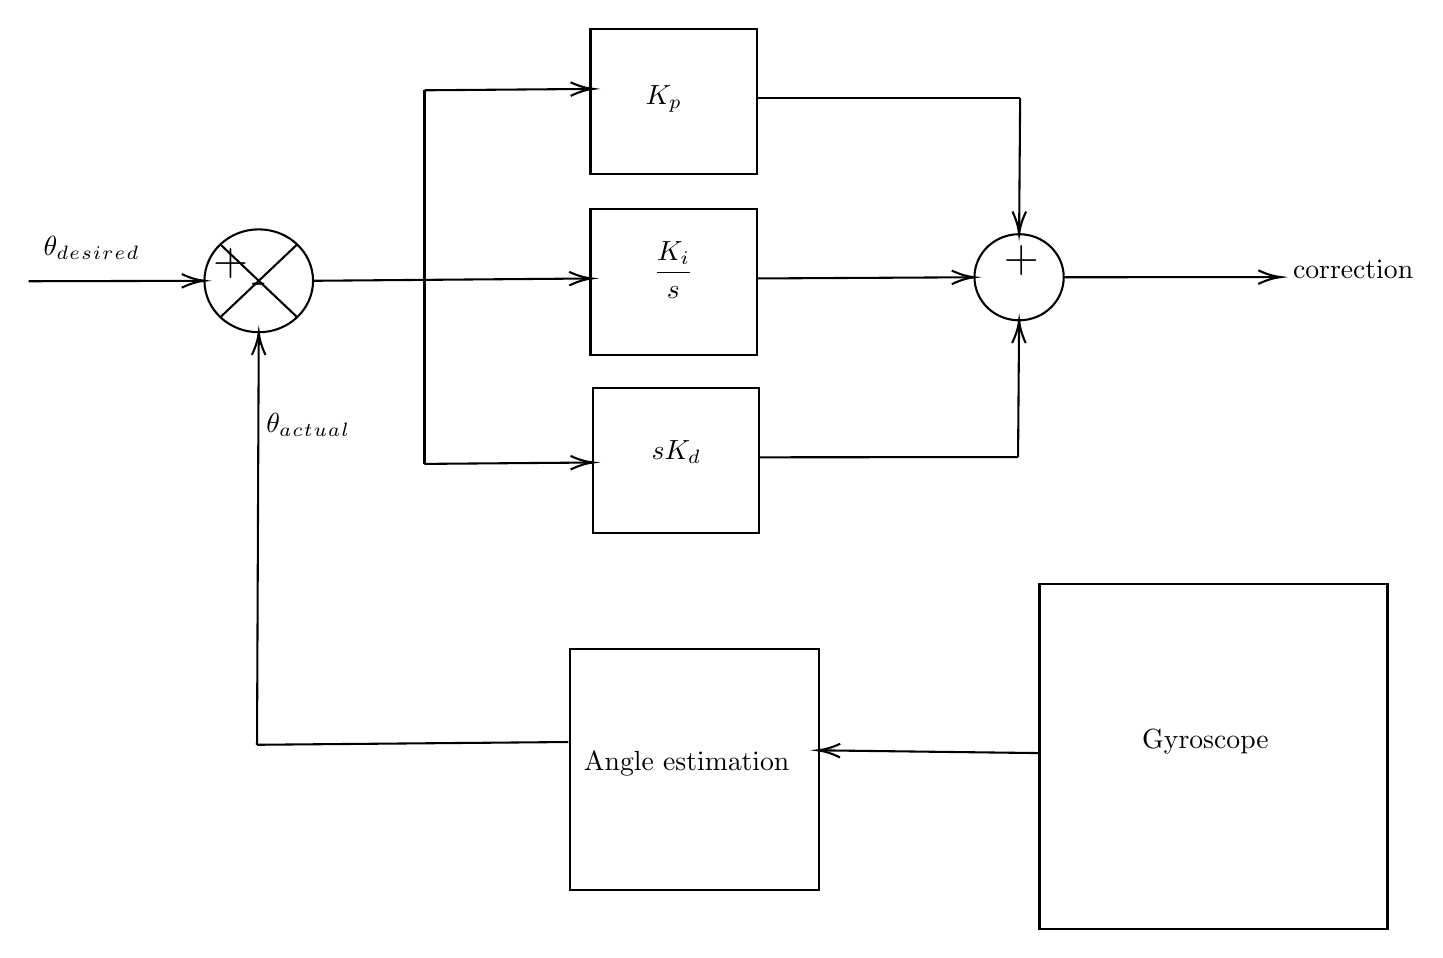
\begin{tikzpicture}[x=0.75pt,y=0.75pt,yscale=-1,xscale=1]
%uncomment if require: \path (0,492); %set diagram left start at 0, and has height of 492

%Flowchart: Process [id:dp850375409387905] 
\draw   (271,16) -- (351,16) -- (351,86) -- (271,86) -- cycle ;
%Flowchart: Process [id:dp8796232359395437] 
\draw   (271,103) -- (351,103) -- (351,173) -- (271,173) -- cycle ;
%Flowchart: Process [id:dp47294256345004837] 
\draw   (272,189) -- (352,189) -- (352,259) -- (272,259) -- cycle ;
%Flowchart: Connector [id:dp24571004653248285] 
\draw   (456,135.75) .. controls (456,124.29) and (465.63,115) .. (477.5,115) .. controls (489.37,115) and (499,124.29) .. (499,135.75) .. controls (499,147.21) and (489.37,156.5) .. (477.5,156.5) .. controls (465.63,156.5) and (456,147.21) .. (456,135.75) -- cycle ;
%Straight Lines [id:da8169341421551133] 
\draw    (351,49.5) -- (478,49.5) ;
%Straight Lines [id:da4502416120302304] 
\draw    (352,222.5) -- (477,222.38) ;
%Straight Lines [id:da6613603234431595] 
\draw    (478,49.5) -- (477.52,113) ;
\draw [shift={(477.5,115)}, rotate = 270.44] [color={rgb, 255:red, 0; green, 0; blue, 0 }  ][line width=0.75]    (10.93,-3.29) .. controls (6.95,-1.4) and (3.31,-0.3) .. (0,0) .. controls (3.31,0.3) and (6.95,1.4) .. (10.93,3.29)   ;
%Straight Lines [id:da33533830767473116] 
\draw    (477,222.38) -- (477.48,158.5) ;
\draw [shift={(477.5,156.5)}, rotate = 90.43] [color={rgb, 255:red, 0; green, 0; blue, 0 }  ][line width=0.75]    (10.93,-3.29) .. controls (6.95,-1.4) and (3.31,-0.3) .. (0,0) .. controls (3.31,0.3) and (6.95,1.4) .. (10.93,3.29)   ;
%Straight Lines [id:da21563686968419837] 
\draw    (351,136.33) -- (454,135.76) ;
\draw [shift={(456,135.75)}, rotate = 179.68] [color={rgb, 255:red, 0; green, 0; blue, 0 }  ][line width=0.75]    (10.93,-3.29) .. controls (6.95,-1.4) and (3.31,-0.3) .. (0,0) .. controls (3.31,0.3) and (6.95,1.4) .. (10.93,3.29)   ;
%Straight Lines [id:da2527424104299858] 
\draw    (499,135.75) -- (601.67,135.67) ;
\draw [shift={(603.67,135.67)}, rotate = 179.95] [color={rgb, 255:red, 0; green, 0; blue, 0 }  ][line width=0.75]    (10.93,-3.29) .. controls (6.95,-1.4) and (3.31,-0.3) .. (0,0) .. controls (3.31,0.3) and (6.95,1.4) .. (10.93,3.29)   ;
%Flowchart: Summing Junction [id:dp9194992637305719] 
\draw   (85,137.45) .. controls (85,123.76) and (96.72,112.67) .. (111.17,112.67) .. controls (125.62,112.67) and (137.33,123.76) .. (137.33,137.45) .. controls (137.33,151.14) and (125.62,162.24) .. (111.17,162.24) .. controls (96.72,162.24) and (85,151.14) .. (85,137.45) -- cycle ; \draw   (92.66,119.93) -- (129.67,154.98) ; \draw   (129.67,119.93) -- (92.66,154.98) ;
%Flowchart: Process [id:dp35094250097069213] 
\draw   (261.33,314.67) -- (381,314.67) -- (381,431) -- (261.33,431) -- cycle ;
%Flowchart: Process [id:dp4176713068822393] 
\draw   (487.33,283.33) -- (655,283.33) -- (655,449.67) -- (487.33,449.67) -- cycle ;
%Straight Lines [id:da8318324211659236] 
\draw    (487,365) -- (382.33,363.69) ;
\draw [shift={(380.33,363.67)}, rotate = 0.72] [color={rgb, 255:red, 0; green, 0; blue, 0 }  ][line width=0.75]    (10.93,-3.29) .. controls (6.95,-1.4) and (3.31,-0.3) .. (0,0) .. controls (3.31,0.3) and (6.95,1.4) .. (10.93,3.29)   ;
%Straight Lines [id:da7770929014028307] 
\draw    (110.33,361) -- (111.16,164.24) ;
\draw [shift={(111.17,162.24)}, rotate = 90.24] [color={rgb, 255:red, 0; green, 0; blue, 0 }  ][line width=0.75]    (10.93,-3.29) .. controls (6.95,-1.4) and (3.31,-0.3) .. (0,0) .. controls (3.31,0.3) and (6.95,1.4) .. (10.93,3.29)   ;
%Straight Lines [id:da6170567584349302] 
\draw    (110.33,361) -- (260.33,359.67) ;
%Straight Lines [id:da9904469301799068] 
\draw    (0.33,137.67) -- (83,137.46) ;
\draw [shift={(85,137.45)}, rotate = 179.85] [color={rgb, 255:red, 0; green, 0; blue, 0 }  ][line width=0.75]    (10.93,-3.29) .. controls (6.95,-1.4) and (3.31,-0.3) .. (0,0) .. controls (3.31,0.3) and (6.95,1.4) .. (10.93,3.29)   ;
%Straight Lines [id:da9994185094703518] 
\draw    (137.33,137.45) -- (269.67,136.35) ;
\draw [shift={(271.67,136.33)}, rotate = 179.52] [color={rgb, 255:red, 0; green, 0; blue, 0 }  ][line width=0.75]    (10.93,-3.29) .. controls (6.95,-1.4) and (3.31,-0.3) .. (0,0) .. controls (3.31,0.3) and (6.95,1.4) .. (10.93,3.29)   ;
%Straight Lines [id:da92990428124362] 
\draw    (191,45.67) -- (270.33,45.02) ;
\draw [shift={(272.33,45)}, rotate = 179.53] [color={rgb, 255:red, 0; green, 0; blue, 0 }  ][line width=0.75]    (10.93,-3.29) .. controls (6.95,-1.4) and (3.31,-0.3) .. (0,0) .. controls (3.31,0.3) and (6.95,1.4) .. (10.93,3.29)   ;
%Straight Lines [id:da7591807394511714] 
\draw    (191,225.67) -- (270.33,225.02) ;
\draw [shift={(272.33,225)}, rotate = 179.53] [color={rgb, 255:red, 0; green, 0; blue, 0 }  ][line width=0.75]    (10.93,-3.29) .. controls (6.95,-1.4) and (3.31,-0.3) .. (0,0) .. controls (3.31,0.3) and (6.95,1.4) .. (10.93,3.29)   ;
%Straight Lines [id:da6585292782151004] 
\draw    (191,45.67) -- (191,225.67) ;

% Text Node
\draw (296,42) node [anchor=north west][inner sep=0.75pt]   [align=left] {$ $$\displaystyle K_{p}$};
% Text Node
\draw (299,213) node [anchor=north west][inner sep=0.75pt]   [align=left] {$\displaystyle sK_{d}$};
% Text Node
\draw (300,117) node [anchor=north west][inner sep=0.75pt]   [align=left] {$\displaystyle \frac{K_{i}}{s}$};
% Text Node
\draw (468.78,119.16) node [anchor=north west][inner sep=0.75pt]   [align=left] {{\LARGE +}};
% Text Node
\draw (608,126) node [anchor=north west][inner sep=0.75pt]   [align=left] {correction};
% Text Node
\draw (87.8,120.27) node [anchor=north west][inner sep=0.75pt]   [align=left] {{\LARGE +}};
% Text Node
\draw (106.5,132.59) node [anchor=north west][inner sep=0.75pt]   [align=left] {{\LARGE -}};
% Text Node
\draw (266.33,362.67) node [anchor=north west][inner sep=0.75pt]   [align=left] {Angle estimation};
% Text Node
\draw (535.33,352.33) node [anchor=north west][inner sep=0.75pt]   [align=left] {Gyroscope};
% Text Node
\draw (113.33,199.73) node [anchor=north west][inner sep=0.75pt]    {$\theta _{a}{}_{c}{}_{t}{}_{u}{}_{a}{}_{l}$};
% Text Node
\draw (6,114.4) node [anchor=north west][inner sep=0.75pt]    {$\theta _{d}{}_{e}{}_{s}{}_{i}{}_{r}{}_{e}{}_{d}$};
\end{tikzpicture}}
\caption{System architecture}
\end{figure}

\section{Experiments}
We use \textit{TiHAN UGV Kit} to perform these experiments. ESP32 as microcontroller and MPU6050 is used as gyroscope. 

After several episodes of tuning the proportionality constants we find that $K_p=30, K_i=2$ and $K_d=1$ gives best performance.


%acknowledgments in the unnumbered footnote on the first page.

%\section*{References}
%
%\begin{thebibliography}{00}
%\bibitem{b1} G. Eason, B. Noble, and I. N. Sneddon, ``On certain integrals of Lipschitz-Hankel type involving products of Bessel functions,'' Phil. Trans. Roy. Soc. London, vol. A247, pp. 529--551, April 1955.
%\bibitem{b2} J. Clerk Maxwell, A Treatise on Electricity and Magnetism, 3rd ed., vol. 2. Oxford: Clarendon, 1892, pp.68--73.
%\bibitem{b3} I. S. Jacobs and C. P. Bean, ``Fine particles, thin films and exchange anisotropy,'' in Magnetism, vol. III, G. T. Rado and H. Suhl, Eds. New York: Academic, 1963, pp. 271--350.
%\bibitem{b4} K. Elissa, ``Title of paper if known,'' unpublished.
%\bibitem{b5} R. Nicole, ``Title of paper with only first word capitalized,'' J. Name Stand. Abbrev., in press.
%\bibitem{b6} Y. Yorozu, M. Hirano, K. Oka, and Y. Tagawa, ``Electron spectroscopy studies on magneto-optical media and plastic substrate interface,'' IEEE Transl. J. Magn. Japan, vol. 2, pp. 740--741, August 1987 [Digests 9th Annual Conf. Magnetics Japan, p. 301, 1982].
%\bibitem{b7} M. Young, The Technical Writer's Handbook. Mill Valley, CA: University Science, 1989.
%\end{thebibliography}


\end{document}
